% Single-policy setup and completed primary-study results.
% Data and figures: ../evaluations/single_policy/.
% Protocol details and task differences: ../SINGLE_POLICY_EXPERIMENTS.md.
\subsection{Single-policy acquisition}
\label{sec:single-policy-experiments}

We study whether supplying a geometric abstraction helps a language-model agent
acquire an executable manipulation policy from a small number of training
rollouts. The agent generates and revises a Python program, which obtains current
observations and executes through a robot interface. Learning changes the
program, while the supplied geometric estimators and operators remain fixed.
This setting tests policy acquisition and generalization to new layouts. Our
separate online experiments study decisions made by the language model during
continuous interaction.

\paragraph{Tasks and environment.}
We use a simulated SO-100 tabletop robot for three tasks: constructing a bridge,
stacking three cubes, and placing a ring over a fixed peg. The bridge uses two
cube foundations, a spanning rectangular beam, and a cylinder placed on the beam.
Stacking requires an ordered three-cube tower. Ring placement requires grasping
material around an opening and moving the opening over the peg before release.
Each task randomizes layouts and color assignments. Test layouts are held out
from training within each study. These experiments evaluate layout generalization
for the specified tasks and object families.

\paragraph{Comparison.}
Base and Full use the same language model, task specification, calibrated RGB-D
access, public robot information, and action interface within each task. Base
can implement numerical perception in its program. Full additionally receives
supplied sensor-grounded geometry and textual feedback; for bridge and stacking,
this includes symbolic references and geometric operators, while the ring
interface exposes opening and wall geometry. Runtime policies cannot access
simulator object poses, dimensions, contacts, or private evaluator state. Both
arms receive task outcomes as training feedback. This comparison evaluates the
supplied geometric interface as a package, including perception, queries, and
feedback.

\paragraph{Training.}
Each task uses five paired training chains. A pair shares five training layouts,
with disjoint training layouts across pairs. Base and Full have separate
persistent language-model contexts in every pair. We use \texttt{gpt-6-astra}
with high reasoning effort and three generated revisions, R1--R3. R0 is an
observation-only scaffold; R1 is the first generated manipulation program. Each
version is run on all five training layouts. The scene resets between rollouts,
and the program executes with local sensing and control without further
language-model calls within a rollout. The agent receives its own training
outcomes, bounded diagnostic feedback, and images under the study's feedback
rule before proposing the next revision. This gives 30 completed program
generations and 200 training slots per task, including R0.

\paragraph{Training-only retention.}
We maintain an incumbent policy to prevent accepted revisions from losing
previously successful training layouts. A candidate replaces the incumbent only
if its training success set is a strict superset of the incumbent's success set.
Ties and proposals that lose an earlier success retain the incumbent. We preserve
every generated candidate and report both raw-candidate and retained-policy
curves. Retention never uses test outcomes, and it does not guarantee monotonic
test performance.

\paragraph{Evaluation.}
After all training chains are complete and their candidates are frozen, every
saved version is evaluated on the same 100 held-out layouts per task. The
resulting matrix contains 4,000 evaluation slots per task:
2 arms $\times$ 5 chains $\times$ 4 versions $\times$ 100 layouts.
Invalid programs count as failed slots. Task success is determined by a private
physical evaluator: bridge and stacking require the prescribed support structure
and a five-second stability check; ring placement requires the peg to pass
through the opening, the ring center to lie below the peg top, release from robot
contact, and a two-second stability check. Test execution makes no language-model
calls and cannot revise or select policies.

\paragraph{Measures and study differences.}
We report success against revision number and cumulative model resources,
together with paired chain variation. The five policies in each arm share the
same 100 test layouts; their 500 evaluations per version are not 500 distinct
layouts. Resource measures include input and output tokens, cached input, image
attachments, model-request time, and rollout cost. The revision budget is matched
within each task; actual token use is measured. All three primary studies withhold
executor source from both arms. Ring uses explicit pad/jaw commands and a different
image-feedback schedule. Bridge and Ring registered the full evaluation matrix
before training; Stacking's expansion from 20 to 100 layouts was post-hoc, without
retraining. Ring preserves two interrupted requests with unknown token usage and
an authorized transport amendment. These differences delimit cross-task comparisons.

\paragraph{Results.}
Table~\ref{tab:single-policy-results} reports policies retained using training
outcomes only. Full achieves higher mean final test success in all three tasks:
65.4\% versus 56.0\% on Bridge, 81.4\% versus 70.8\% on Stacking, and 38.0\%
versus 0\% on Ring. On Bridge and Stacking, Full's R2 mean already exceeds Base's
R3 mean, suggesting earlier acquisition in these runs. Ring's gains appear only
at R3 and are concentrated in three of five chains; the remaining two retain
zero-success policies. Full is ahead in four Bridge pairs and three Stacking
pairs, so the mean gains do not imply improvement in every training chain.

\begin{table}[t]
\centering
\small
\begin{tabular}{llrrrr}
\hline
Task & Arm & R1 & R2 & R3 & Tokens (k) \\
\hline
Bridge & Base & 21.2 & 53.0 & 56.0 & 125.7 \\
       & Full & 45.2 & 63.4 & 65.4 & 127.0 \\
Stacking & Base & 17.2 & 53.6 & 70.8 & 138.1 \\
         & Full & 57.2 & 72.2 & 81.4 & 123.4 \\
Ring & Base & 0.0 & 0.0 & 0.0 & 166.8 \\
     & Full & 0.0 & 0.0 & 38.0 & 163.1 \\
\hline
\end{tabular}
\caption{Training-retained test success (\%) averaged over five paired chains,
with 100 shared test layouts per task. Tokens are mean cumulative completed-request
input plus output tokens per chain through R3, including rejected proposals.
Ring Base excludes unknown usage from two interrupted requests. R0 is an
observation-only scaffold with zero success in both arms.}
\label{tab:single-policy-results}
\end{table}

Raw R3 means are 56.0\%/66.0\% for Bridge, 70.8\%/81.4\% for Stacking, and
0\%/38.2\% for Ring (Base/Full). Retention never substitutes a candidate based
on a favorable test result. On Stacking's additional 80 layouts alone, retained
R3 success is 69.5\%/79.5\%. Full's completed-token consumption is 1.0\% higher
on Bridge, 10.6\% lower on Stacking, and 2.2\% lower on Ring; these results do
not establish a uniform token-saving effect. Ring's interrupted requests add
1,800 seconds of aggregate request time with unknown tokens. Acquisition cost
and trained-policy success are distinct from online reasoning latency.

% Requires graphicx. Paths assume this fragment is compiled from docs/paper/.
\begin{figure*}[t]
\centering
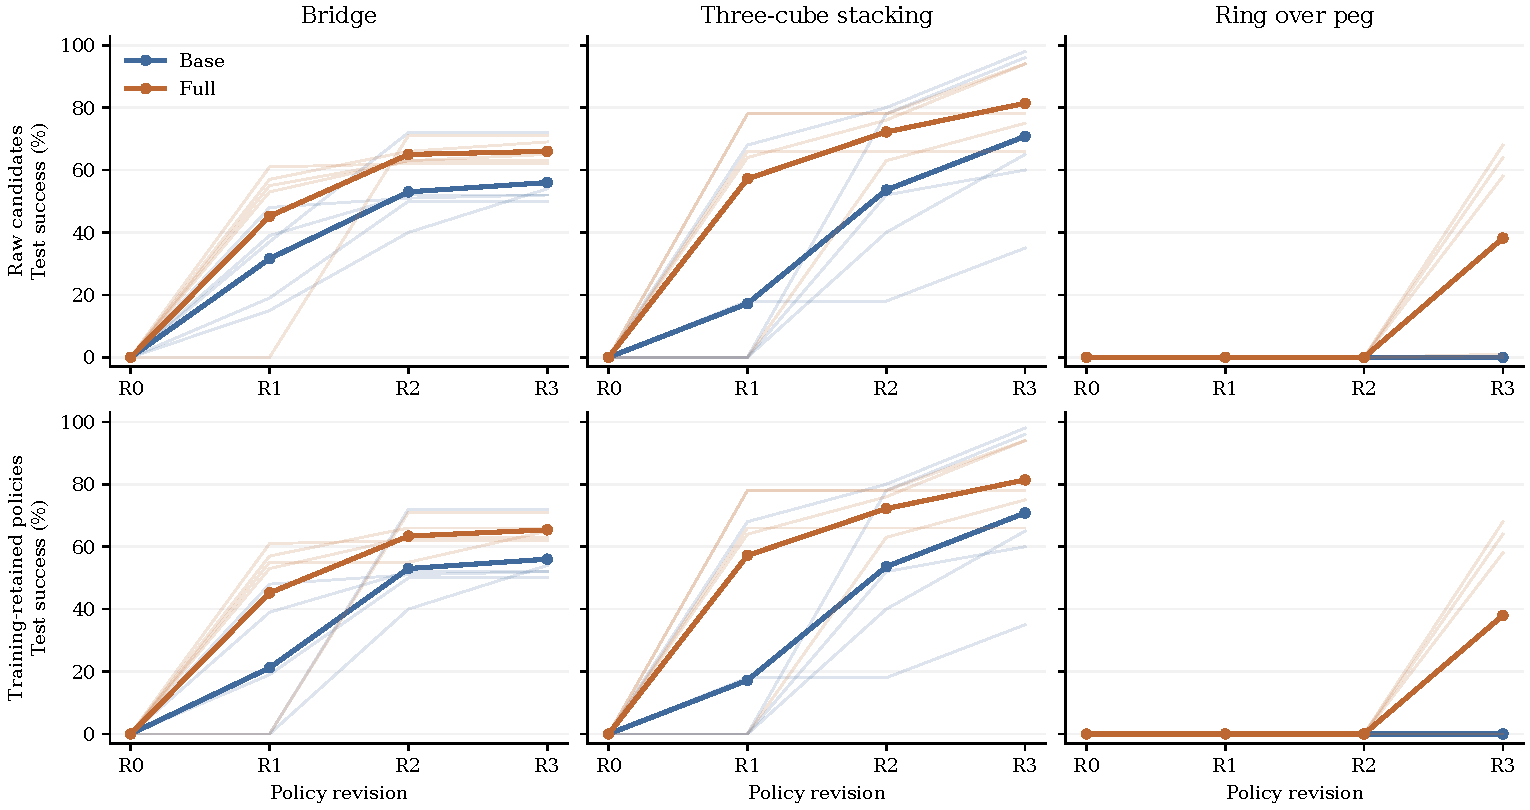
\includegraphics[width=\textwidth]{../evaluations/single_policy/learning_curves.pdf}
\caption{Single-policy acquisition. Top: raw candidates. Bottom: policies
retained using strict improvement of the training success set. Bold lines show
means over five paired training chains; faint lines show individual chains.
Every version is evaluated on the same 100 held-out layouts per task after
training freezes. R0 only observes; R1 is the first generated manipulation
program. No test outcome is used for policy retention.}
\label{fig:single-policy-curves}
\end{figure*}

\paragraph{Scope.}
These small replicated studies evaluate layout generalization within specified
tasks and object families, with the supplied geometry interface treated as a
package. The shared test layouts are crossed with five trained policies; their
500 outcomes per arm/version are not 500 independent layouts. The frozen Bridge
and Stacking evaluators use a historical contact helper that can miss unnamed
robot collision geometry; Ring uses body-ancestry contact checks. Ring's nominal
12\,mm lateral clearance also limits interpretation as precision insertion.
